\chapter{Protocol Design}
\label{chap:protocoldesign}

In the state of the art, there are different protocols constructed over \ac{IEEE} 802.15.4, like ZigBee, WirelessHART, 6LoWPAN \ldots \ some
are prepared for low consumption, others build different applications, but almost none of them are focused in localization. In the
department \ac{LPL} and \ac{OLP} \cite{LPLandOLP} protocols were proposed for this purpose. This protocols are based in \ac{IEEE} 802.15.4 and specifically 
designed for localization. In the next section a brief overview will be given, for a deeper view, please consult \cite{LPLandOLP}.

\section{\ac{LPL} and \ac{OLP}}

\ac{LPL} and \ac{OLP} \cite{LPLandOLP}, are two protocols designed for localization and based in \ac{RSSI} values. This values give an idea of 
the received signal strength in the device, and have the advantage that this information is already in all packets a device receives, there
is no need of special hardware or data to be prepared or obtained like in other methods (ultra wide band for example). But \ac{RSSI} values have 
a big problem for localization, its dispersion is very big, making the localization resolution (in some cases up to many meters 
\cite{fingerprint}) bad for some applications. 

This resolution problem, can be solved through some approaches. One kind is using localization techniques like ``fingerprint 
technique'' \cite{fingerprint} that improves the resolution. Another option is, taking more than 1 \ac{RSSI} value to obtain a more stable 
result. This technique has one big challenge, the more values are taken, the higher the energy consumption. Without a good approach, 
the \ac{MN} would need to listen to the channel most of the time waiting to receive packets from \ac{AN} to obtain \ac{RSSI} values, 
this way a lot of energy would be wasted just doing nothing, this is called idle listening. This 2 protocols propose 2 different 
approaches to solve this.

Another aspect in localization is who calculates the position, 3 different alternatives can be obtained.

\begin{itemize}
 \item \textbf{Centralized.} A central computer receives the \ac{RSSI} values from all \acp{AN} in the network and calculates the positions of 
the \acp{MN}. The advantage is that the computer can use complicate algorithms to obtain better results, but this method 
charges the network with a lot of traffic, specially if the \ac{MN} needs to know its position back after calculation.
 \item \textbf{Distributed-A.} The \ac{MN} sends the \ac{RSSI} values directly to the \ac{AN}, and this calculates directly the \ac{MN} position,
this does not charge the network so much like the centralized approach but the resolution is also not so good. It is important to note that 
each \ac{MN} has a ``selected \ac{AN}'', this \ac{AN} is the one in charge to calculate \ac{MN} position and the one the \ac{MN} communicates
with and through. This \ac{AN} is usually the one closest to the \ac{MN}.
 \item \textbf{Distributed-M.} In this mode, is the \ac{MN} who calculates directly its position from \ac{RSSI} values obtained from \acp{AN},
the problem is that \acp{MN} cannot use powerful localization algorithms. This solution is the one that almost does not charge the network.
\end{itemize}

The protocols \ac{LPL} and \ac{OLP} are going to use phases for different behaviors, and this phases will be repeated cyclically, that's why 
a good synchronization among all the nodes is necessary so all nodes can start the phases at the same time. Nodes will get 
the synchronization information from their parents (do not forget that a tree topology is used) using an active or a passive synchronization. 
To get a graphical explanation check Figure \ref{fig:synchronization}.

\begin{itemize}
 \item \textbf{Passive Synchronization.} The parent starts the process sending a packet R1 to \ac{MAC} to be transmitted, this packet is
created at the time-stamp Tx1, and includes this time, the time until the next phase start (TF) and info about this phase. Due to random time in 
\ac{CSMA/CA} process and other processing times, R1 is not transmitted immediately but in Tx2. When the packet is transmitted, \ac{MAC} informs
the application layer and this creates another packet (R2) including the new time-stamp Tx2. At the child, 2 packets will be received, R1 and 
R2 in times Rx1 and Rx2 respectively. Calculation of next phase start from the child point of view (TZ) is done like in (\ref{mat:pasivesync}).

\begin{equation}
  TZ = TF - (Rx2 - Rx1) - (Tx2 - Tx1)
  \label{mat:pasivesync}
\end{equation}

\begin{figure}[here]
 \begin{center}
  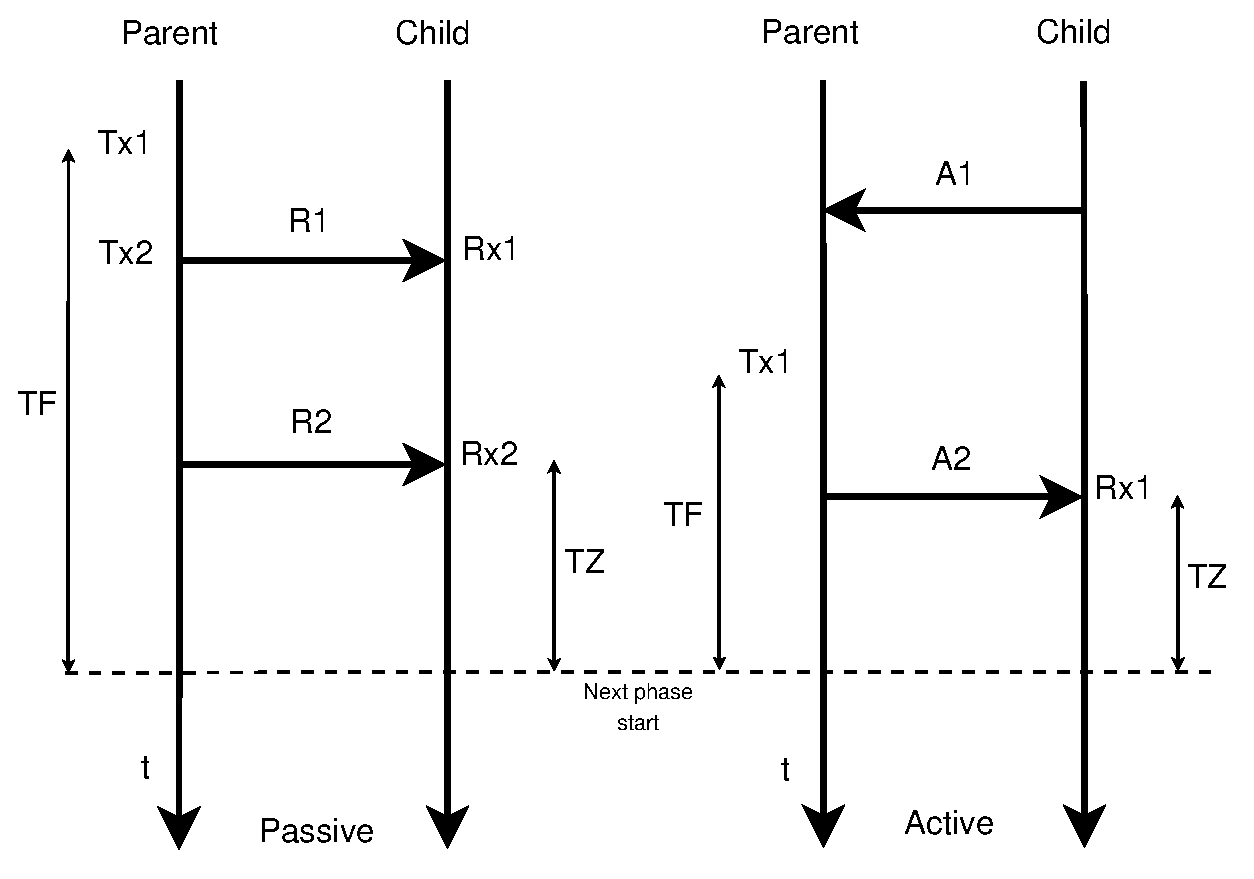
\includegraphics[width=0.6\textwidth]{synchronization.eps}
 \end{center}
 \caption{Passive and Active Synchronization \cite{LPLandOLP}}
 \label{fig:synchronization}
\end{figure}
 
 \item \textbf{Active Synchronization.} In the active synchronization, the child starts the process sending a synchronization request (A1),
then the parent answers with packet A2, this packet contains the time until the start of the next phase (TF). The child can calculate this time
with like in (\ref{mat:activesync}).

\begin{equation}
  TZ = TF - C
 \label{mat:activesync}
\end{equation}

The C parameter in (\ref{mat:activesync}), represents an estimation of all the processing times and random times from \ac{CSMA/CA}, that is why
this method is not so exact like the passive one, although it does not need 2 packets like it.
\end{itemize}

In the following subsections, both protocols \ac{LPL} and \ac {OLP} are going to be introduced.

\subsection{\acl{LPL}}

To reduce the idle listening, and thus the energy consumption, this protocol, proposes that instead of listening to the \acp{AN}, the
\acp{MN} are the ones who transmit and the \acp{AN} the ones who listen and transmit this information. This protocol is divided in 3 
phases which can be appreciated in Figure \ref{fig:LPL}.

\begin{figure}[h]
 \begin{center}
  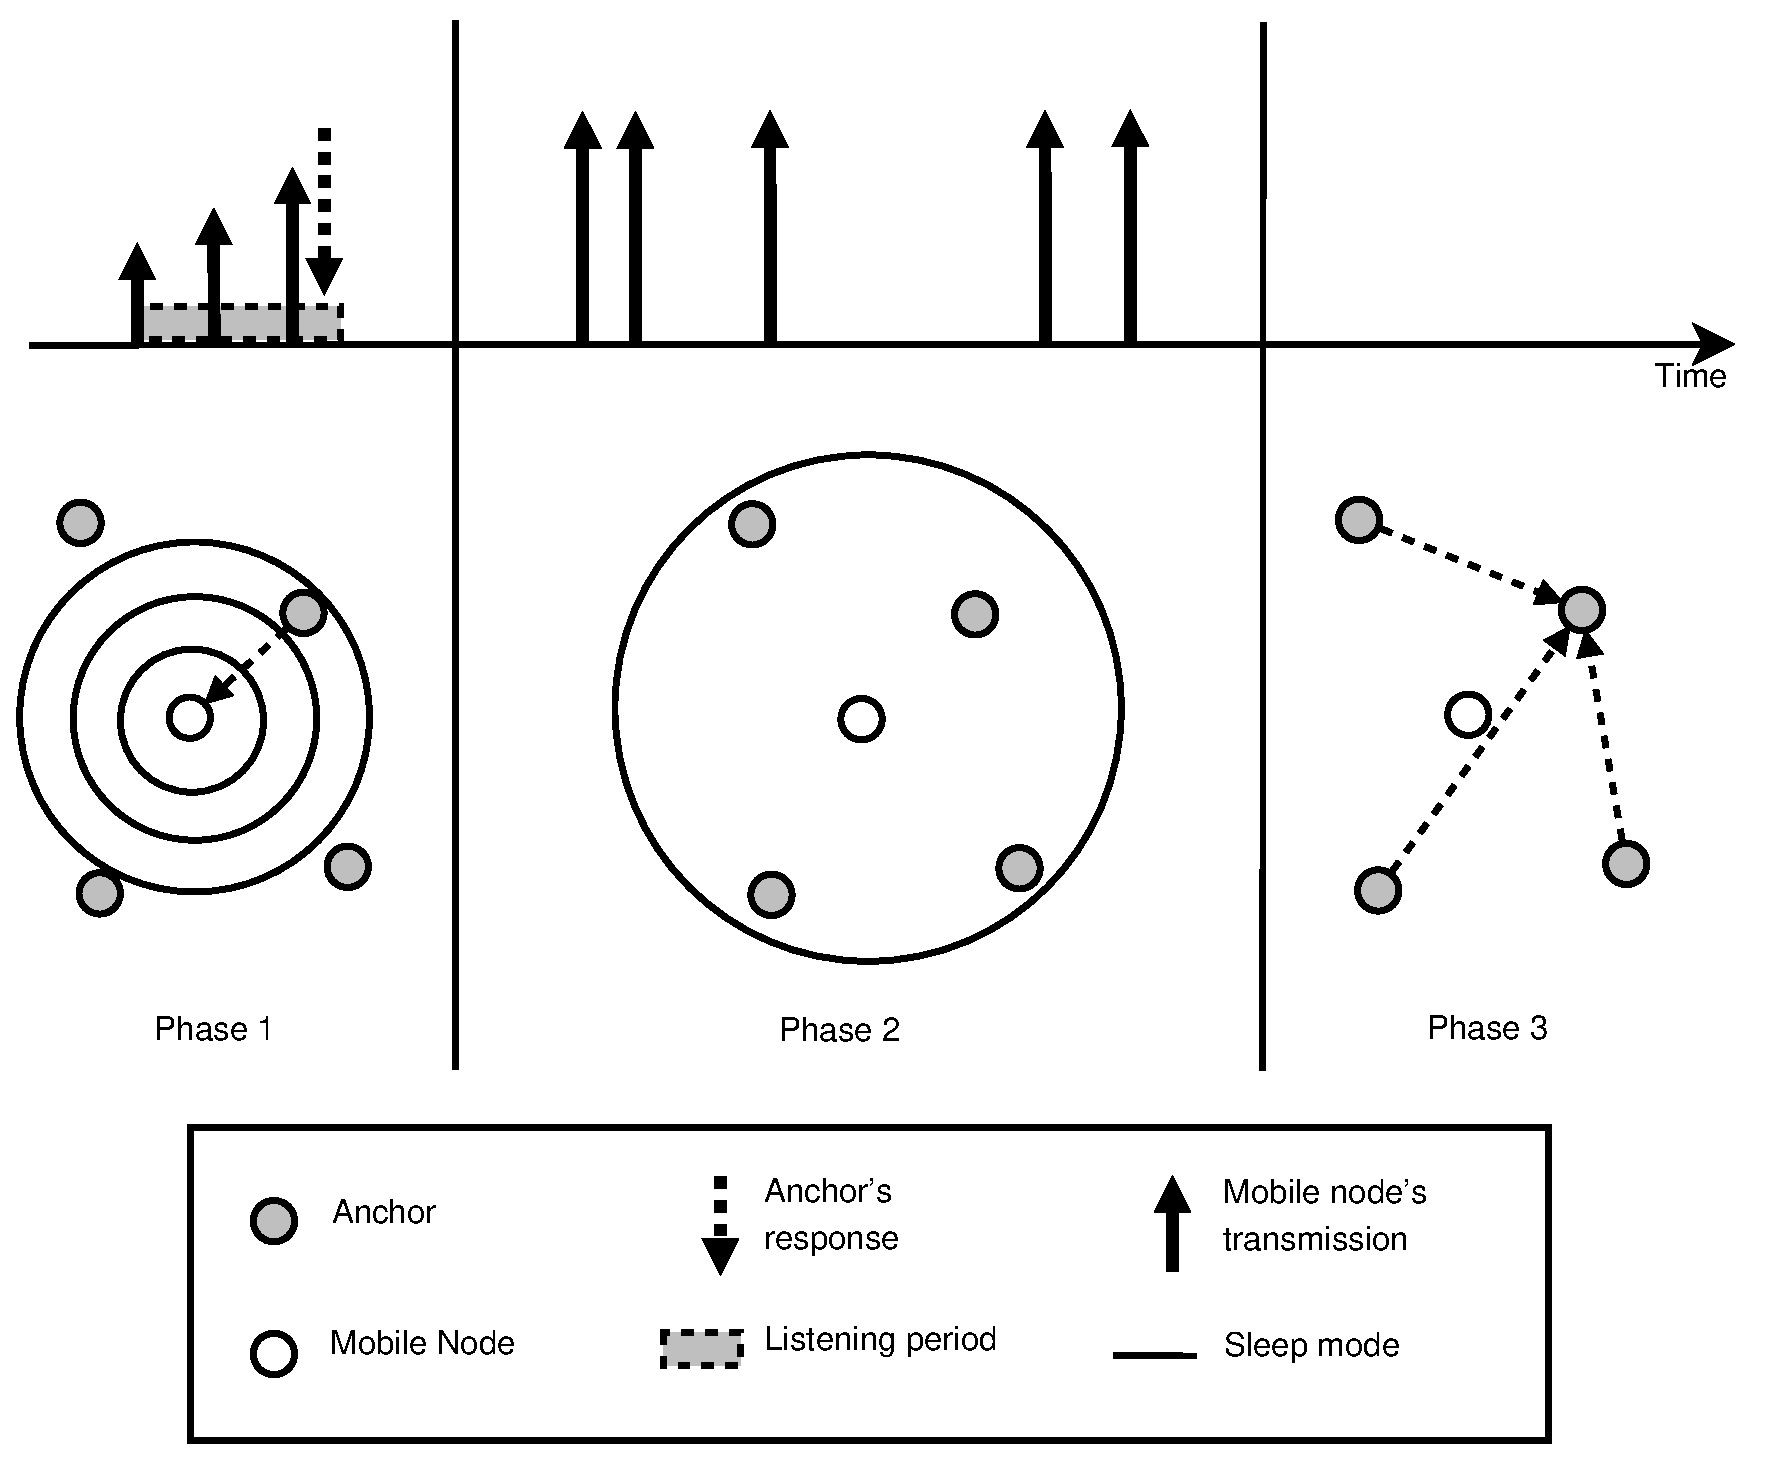
\includegraphics[width=0.7\textwidth]{LPL.eps}
 \end{center}
 \caption{LPL Phases \cite{LPLandOLP}}
 \label{fig:LPL}
\end{figure}

\begin{itemize}
 \item \textbf{Phase 1:} In this phase, \ac{MN} selects a random time to broadcast a synchronization request, starting with the minimum power,
and increasing this power until it receives an answer from an \ac{AN}, this will be the selected \ac{AN}, and the answer will contain information
about the phase times. This process makes sure that only the nearest \acp{AN} answer to this synchronization request. In the next phase 1, if 
the \ac{MN} needs to know its position, it asks its selected \ac{AN} about this information, and if not it just synchronizes.
 \item \textbf{Phase 2:} In phase 2, the \ac{MN} broadcasts several packets in random times to minimize the collisions. Any time the node is not
transmitting, it goes to sleep, this makes that \acp{MN} are awake only when they transmit eliminating this way the idle listening. The \acp{AN} that
received this broadcasts, store the read \ac{RSSI} values and the selected \ac{AN}.
 \item \textbf{Phase 3:} During this phase, the \acp{MN} sleeps and the \acp{AN} send the measured \ac{RSSI} values to the selected \ac{AN}. 
This \ac{AN} will calculate the \ac{MN} position in Distributed-A case or send the data to a central computer in Centralized case. In this phase is
also done the synchronization between \acp{AN} and network configuration.

This protocol, has some problems that make it not suitable for all conditions:

\begin{itemize}
 \item Hidden Terminal Problem. This problem is here strong not only because it could make big idle listening in phase 2, but it could also 
happen that, if 2 \acp{MN} transmit at the same time, the selected \ac{AN} might not be the one closest to the \ac{MN} but one with a not so 
good connection.
 \item High \ac{MN} number. If the number of \acp{MN} is high, phase 2 is going to be full of collisions and thus, the idle listening will be
high. In phase 1, the hidden terminal problem would be stronger.
 \item Selected \ac{AN} selection. If many \acp{AN} are close to the \ac{MN}, all of them are going to try to answer causing collisions. Also, 
when the \acp{AN} are not close to the \ac{MN}, a lot of energy is wasted in the \ac{MN} trying to detect gradually the selected \ac{AN}.
\end{itemize}


\end{itemize}


\subsection{\acl{OLP}}

In the case of \ac{OLP} protocol and unlike \ac{LPL}, the \ac{MN} is the one who listens. This protocol is also divided in 3 phases, 2 of 
them can be appreciated in Figure \ref{fig:OLP}.

\begin{figure}[ht]
 \begin{center}
  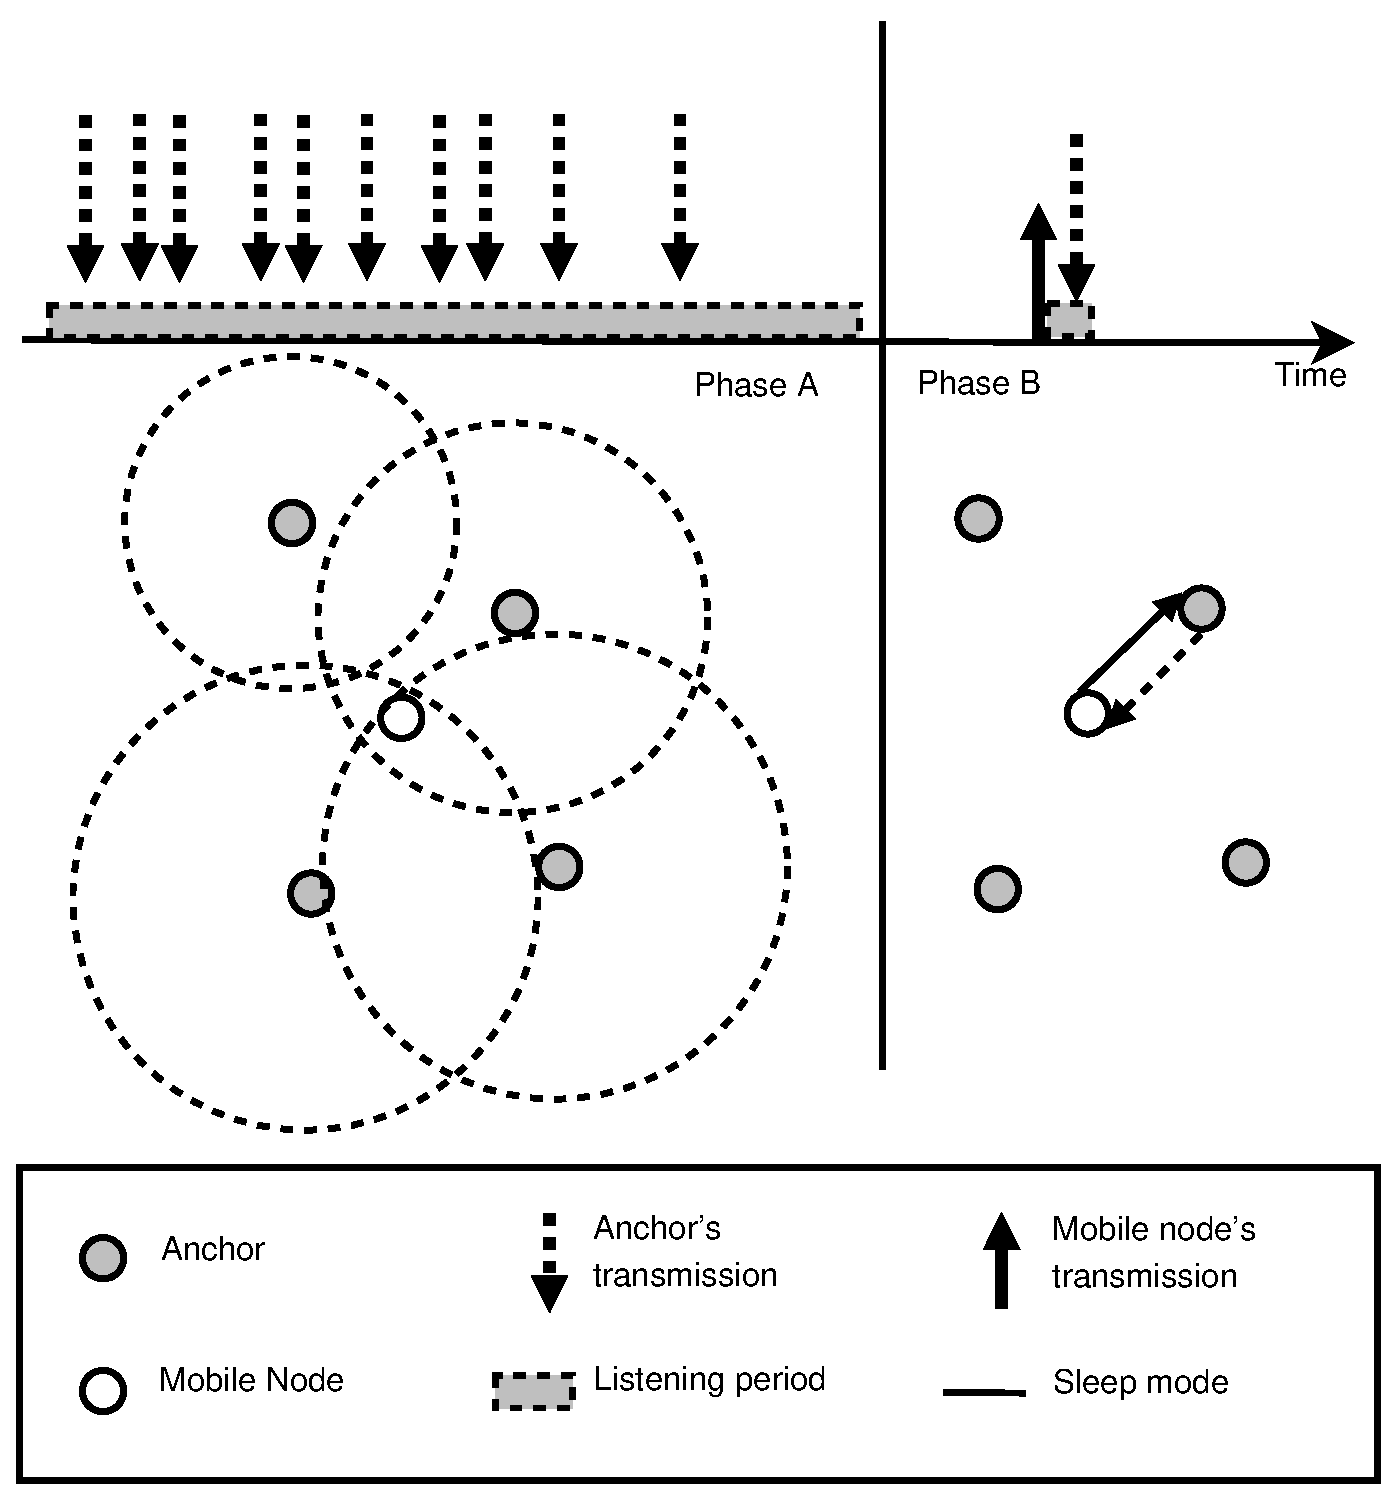
\includegraphics[width=0.55\textwidth]{OLP.eps}
 \end{center}
 \caption{OLP Phases \cite{LPLandOLP}}
 \label{fig:OLP}
\end{figure}

\begin{itemize}
 \item \textbf{Phase A:} In this phase, and thanks to the synchronization among \acp{AN}, the inter-arrival time is reduced, reducing so the
idle listening. This packets also content synchronization information for the \ac{MN}. In this phase \ac{RSSI} values are received and stored
by the \ac{MN}, and then it goes to sleep.
 \item \textbf{Phase B:} In this phase and in Distributed-M mode, the \ac{MN} will use easy localization algorithms together with all the \ac{RSSI}
values read to get its position. In case of Distributed-A or Centralized mode, the \ac{MN} will send a report to the selected \ac{AN}, took 
from the highest \ac{RSSI} value, with all the stored \ac{RSSI} values in Phase A. The selected \ac{AN} will answer with an \ac{ACK}. In next
phase B, the \ac{MN} will ask the selected \ac{AN} about its position in case it needs it.
 \item \textbf{Phase C:} Like in \ac{LPL} this Phase is reserved for communication among \acp{AN} and network configuration.
\end{itemize}

\ac{OLP} has also some problems:

\begin{itemize}
 \item Synchronization. In this protocol, a really good \acp{AN} synchronization is needed to make the idle listening in phase 1 from the 
\acp{MN} as low as possible. This is not easy, specially with a tree structure where the synchronization error will be increased and 
propagated through the tree.
 \item \ac{MN} listens too much. The \ac{MN} is listening during long periods of time where all the \acp{AN} are transmitting, some times it
could even happen that the \ac{MN} it is not at a reachable distance from the \ac{AN} that is transmitting, listening in this moment just 
for nothing.
 \item Hidden Terminal Problem. If the \acp{AN} are not good synchronized to avoid this problem, the \acp{MN} would get many invalid 
packets, being this a waste of energy. If the number of \acp{MN} is big, then in phase 2 we could have many collision problems.
 \item Temporal \ac{RSSI} Correlation. As the \ac{RSSI} values are very correlated in near times \cite{RSSIcorrelated}, receiving all 
the packets so close in time would not contribute to have a better and more stable \ac{RSSI} measurement.
\end{itemize}
 

\section{High Configurable Protocol proposal}

From the previous section and according to the results in \cite{LPLandOLP}:
\begin{quote}
``LPL consumes lower energy than OLP when many RSSI samples are required from many ANs. On the other hand,
OLP becomes more energy efficient than LPL when there are several MNs and few RSSI samples are needed.''\cite{LPLandOLP}
\end{quote}

From this, it could be extracted that depending on the application, and the network load, it could be better that some nodes could have a 
configuration where their main action is listening and others could have a configuration where their main action is broadcasting. This 
configuration should be variable depending on the current network situation and the necessities of the node. From this, arises the necessity
of a High Configurable Protocol with different node configurations.

\subsection{Node Configurations}

From the Table \ref{tab:wsn_applications} (page~\pageref{tab:wsn_applications}) where different applications for \ac{WSN} where stated and the
previous paragraph, it is possible to extract this 4 different node configurations.

\begin{itemize}
 \item \textbf{Mode 1.} This is the normal configuration, when the \ac{MN} does not have any special need. A \ac{MN} with this configuration,
will listen to the \acp{AN} and then send the selected \ac{AN} a packet with the measurements. This is equivalent to having just \ac{OLP}. This
configuration supports the Centralized and Distributed-A working modes.
 \item \textbf{Mode 2.} This configuration mode is similar to mode 1, but in this case is prepared to work only with Distributed-M working mode.
From time to time in case it's needed, it could send the estimated positions to its selected \ac{AN}.
 \item \textbf{Mode 3.} This configuration, also called \ac{VIP} mode, is used when the node is in a critical situation respecting the battery.
This configuration is similar to \ac{LPL} where the \ac{MN} broadcasts and the \acp{AN} receive the packets and send them to a coordinator that
will be able to estimate \ac{MN} position. When it is needed, a way for the \ac{MN} to request its position is provided, this will be explained 
later. 
 \item \textbf{Mode 4.} Unlike the previous configuration, this configuration is for nodes without battery problems, and with a high accuracy
need or a big urgency. This configuration is a mix of mode 1 and 3, the \ac{MN} listens to the \acp{AN} broadcasts but also they broadcast their
self packets to be measured by the \acp{AN}, all this information together is sent to a coordinator that will estimate \ac{MN} position.
This node loads the network so much and will be used just when strictly needed.
\end{itemize}

This is just a brief description of the different configurations. As the protocol is yet to be explained, a full behavior description from 
every configuration will be done later together with the protocol description.

\subsection{Protocol Description}

From previous section, it is obtained that this protocol, needs at least 3 different phases to work. One of the phases is Sync 
Phase, where the \acp{AN} will transmit broadcasts and the \acp{MN} will listen to get \ac{RSSI} values and synchronize. Another needed 
phase is a phase where \acp{AN} and \acp{MN} could communicate among them. And the last needed phase, is a phase where the \acp{AN} could 
communicate with each other to and from the coordinator.

\acp{MN} configured with mode 3, are nodes with critical battery. This nodes cannot waste energy, and this means their idle listening must be
as low as possible. As this nodes will not waste time listening and will just transmit broadcasts, it could be interesting reserving a phase
just for them, where their transmissions will not interfere with the ones from the rest of the \acp{MN}, this phase will be called \ac{VIP} 
Phase. It is clear, that the number of \ac{VIP} \acp{MN} cannot be too big as this way, their exclusivity will not be anymore exclusive.
This phase should not be so long as there are still many other \acp{MN} to transmit and the phases collection would become too long.
The phase for communication among \acp{MN} and \acp{AN} will be named Report Phase, and here is where Mode 4 \acp{MN} can make 
their broadcasts and where communication among \acp{MN} and \acp{AN} can take place.

The main purpose of the phase where \acp{AN} communicate with each other, is to transmit information between the coordinator or sink and 
the \acp{MN}. That is the reason why this phase will be called ComSink Phase. This phase should be the biggest one, as all traffic from 
the \acp{MN} should reach the sink and come back, and all \acp{AN} must transmit their own \acp{MN} information and route the one coming from
their sons or parents. As the traffic in this phase will be high, its useful to distinguish between up-links traffic and down-links traffic, 
ComSink Phase will be divided in ConSink Phase 1 (up-links) and ComSink Phase 2 (down-links).

As it was said, \ac{RSSI} values are very correlated in near times \cite{RSSIcorrelated}, that is why it could be favorable to distribute the 
Sync Phase to get better \ac{RSSI} samples. As apart from Sync Phase, the protocol consists in Report Phase, \ac{VIP}
Phase, ComSink Phase 1 and ComSink Phase 2, if Report Phase and \ac{VIP} Phase are scheduled together, Sync Phase can be divided into 3
separated in time phases, Sync Phase 1, Sync Phase 2 and Sync Phase 3. This sync phases will be intercalated between the other phases.

This phase collection will be repeated in time, being the period every phases collection repetition. For a better understanding of this 
phase division, check Figure \ref{fig:ProtocolPhases}. This Figure will be explained in detail later.

\begin{figure}[ht]
 \begin{center}
  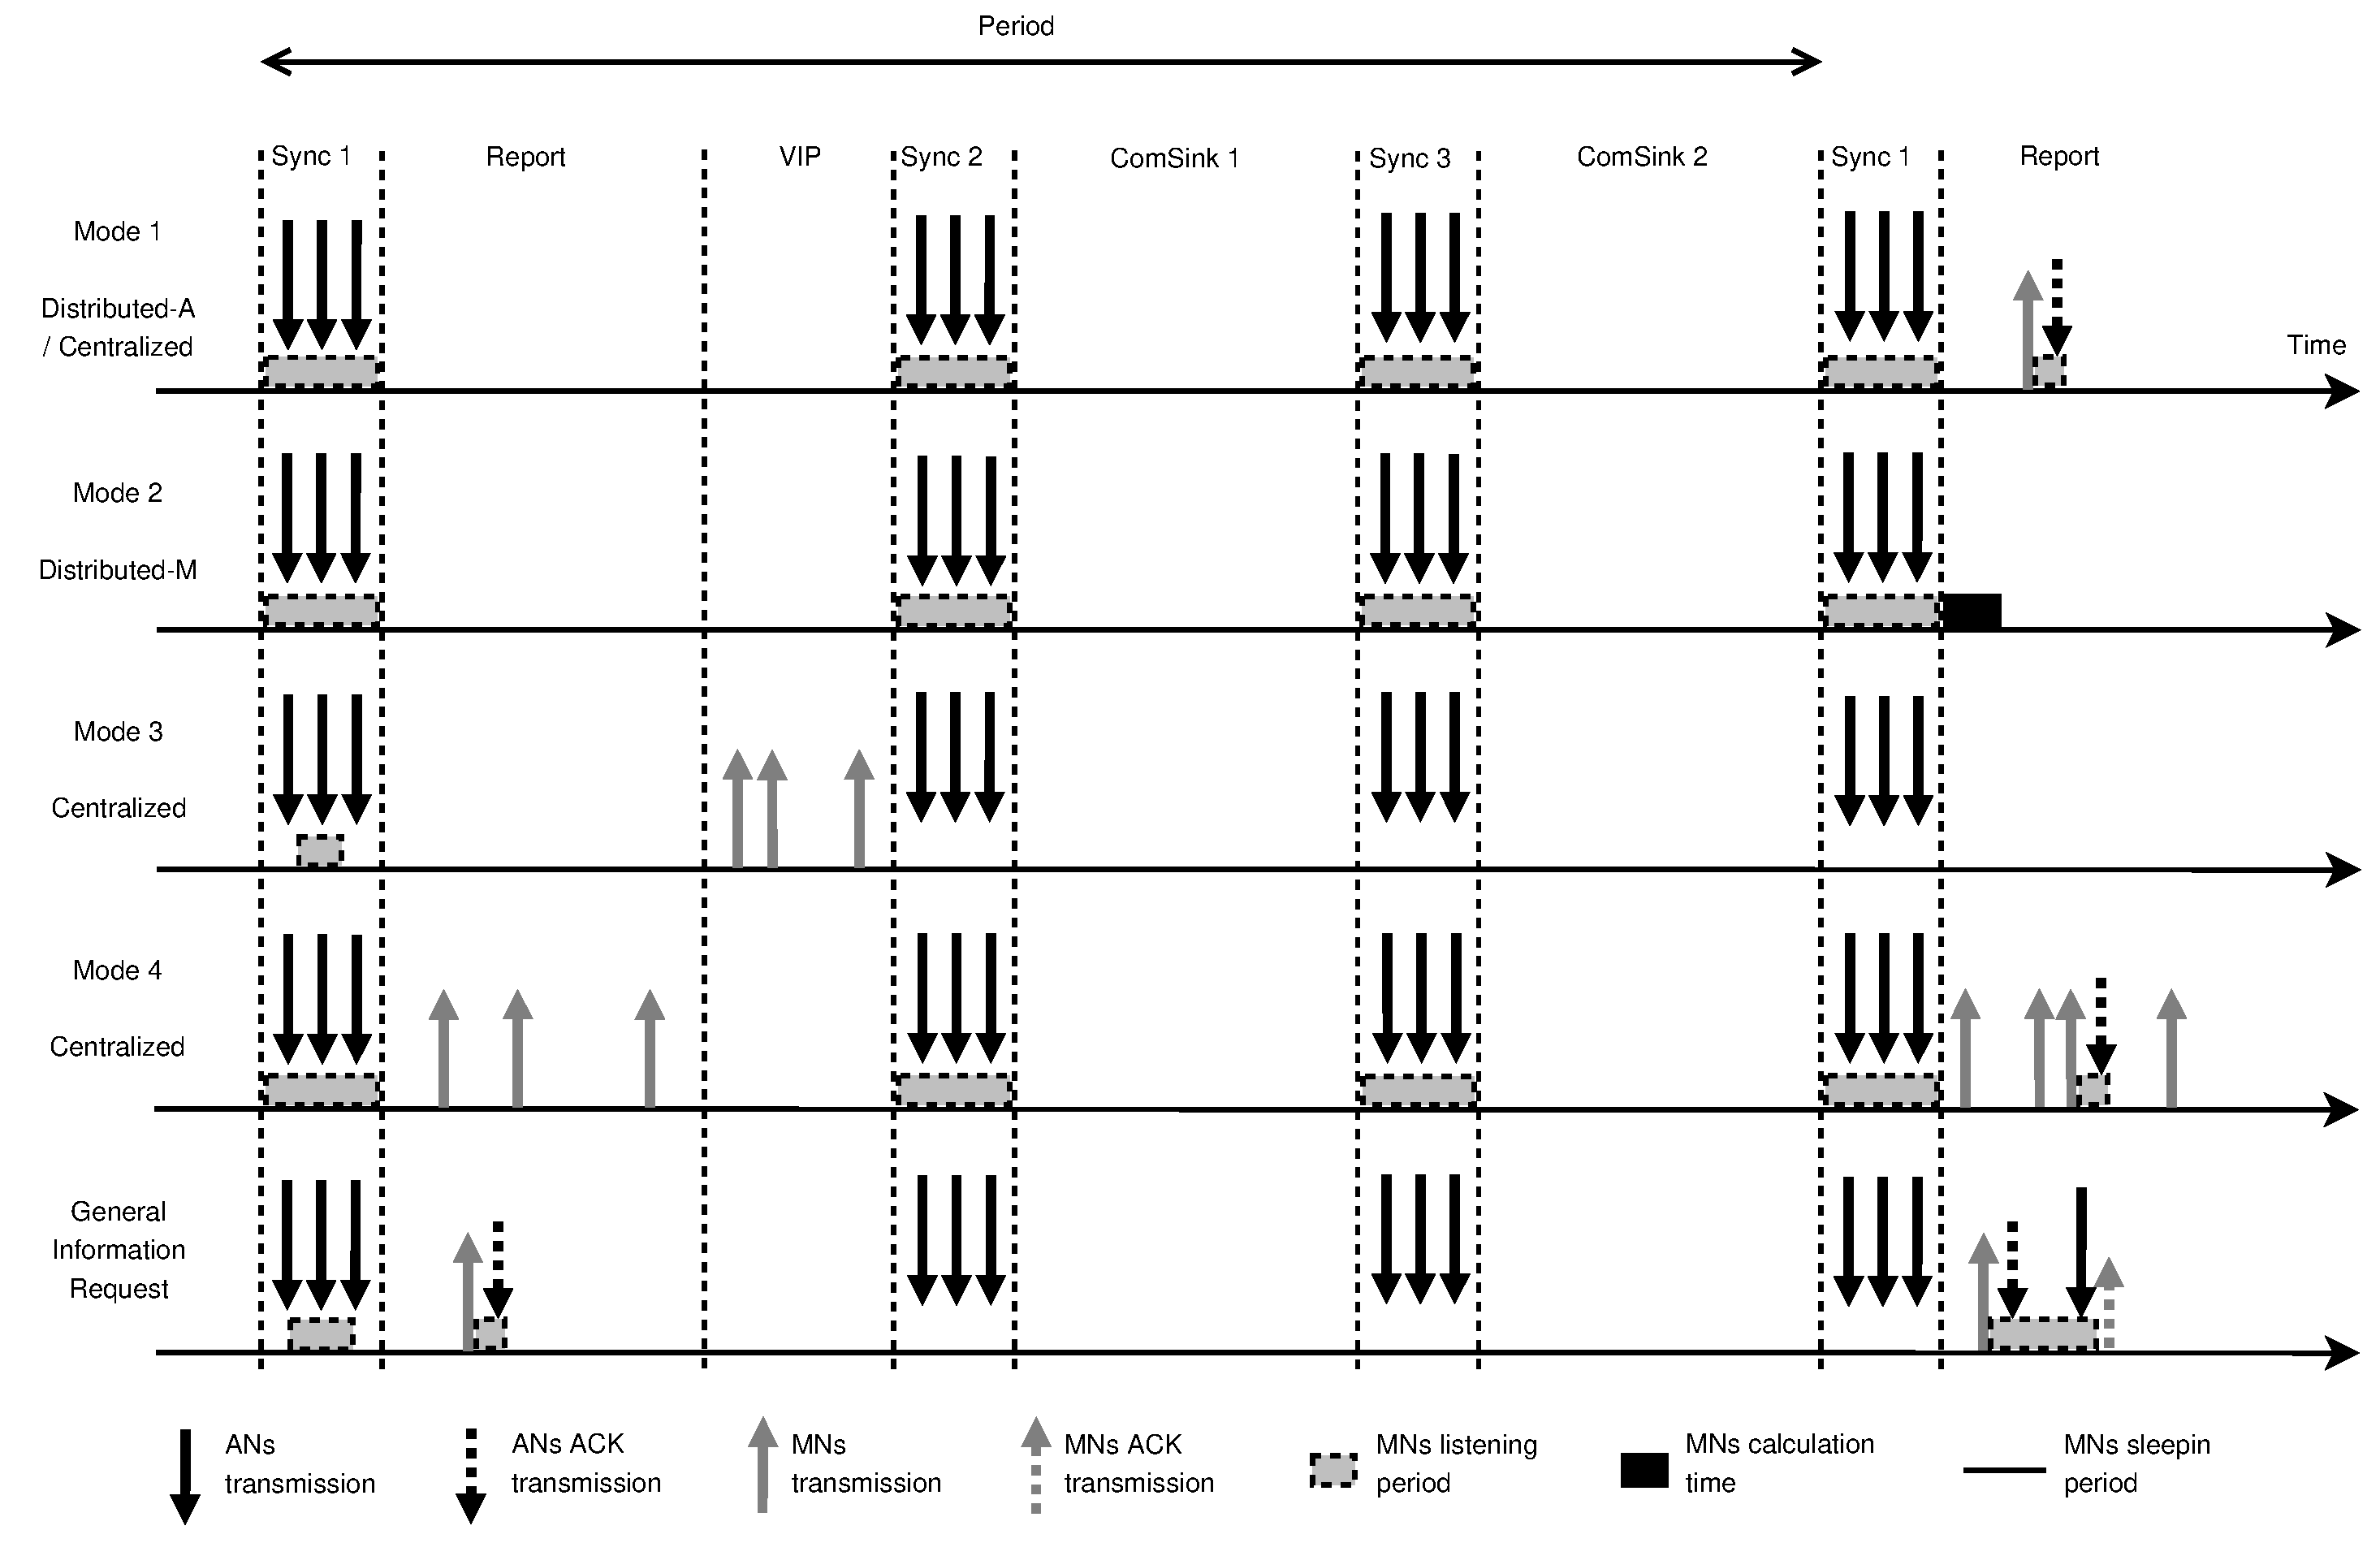
\includegraphics[width=1\textwidth]{ProtocolPhases.eps}
 \end{center}
 \caption{High Configurable Protocol Phases \cite{mipaper}}
 \label{fig:ProtocolPhases}
\end{figure}

The Figure \ref{fig:ProtocolPhases} is divided into 5 sections, one per Configuration Mode and the last one for explaining the General Information
Request. To understand properly how the protocol works, this sections have to be explained in detail:

\begin{itemize}
 \item \textbf{Mode 1.} This \acp{MN} listen during the Sync Phases to the \acp{AN} broadcasts, here they take the \ac{RSSI} values and send them
to their selected \ac{AN}, this is obtained from the highest measured \ac{RSSI}. The selected \ac{AN} answers with an \ac{ACK} to the \ac{MN}.
 \item \textbf{Mode 2.} 
 \item \textbf{Mode 3.} 
 \item \textbf{Mode 4.} 
 \item \textbf{General Information Request.} 
\end{itemize}

Here, it is just defined the standard behavior of the different configurations, but to really extract a high configuration of the protocol, some 
parameters must be taken into account.

\begin{itemize}
 \item \textbf{activePhases -} This are the periods where the \ac{MN} is active with its standard behavior (already commented).
 \item \textbf{inactivePhases -} This are the periods where the \ac{MN} is sleeping.
 \item \textbf{offsetPhases -} This are the periods to leave inactive before the first active period comes.
 \item \textbf{offsetSyncPhases -} This are the Sync Phases where \acp{MN} don't listen in the first active phase, will be explained later.
 \item \textbf{reportPhases -} This is the periods frequency where the \ac{MN} can send an extra report to the \ac{AN}, even if it is 
an inactive period.
 \item \textbf{askFrequency -} This is the extra report frequency when a flag will be activated in the extra report from a \ac{MN} to 
an \ac{AN}, to indicate the \ac{AN} that next phase some information will be requested.
 \item \textbf{offsetReportPhases -} This are the periods to leave before the first extra report is scheduled.
\end{itemize}
 
As an example to explain this parameters check Figure \ref{fig:parametersphases}, where the parameters take the following values: 

\begin{quote}
 activePhases = 2 | inactivePhases = 2 | offsetPhases = 1 | offsetSyncPhases = 1 | reportPhases = 3 | askFrequency = 2 | offsetReportPhases = 0
\end{quote}

\begin{figure}[ht]
 \begin{center}
  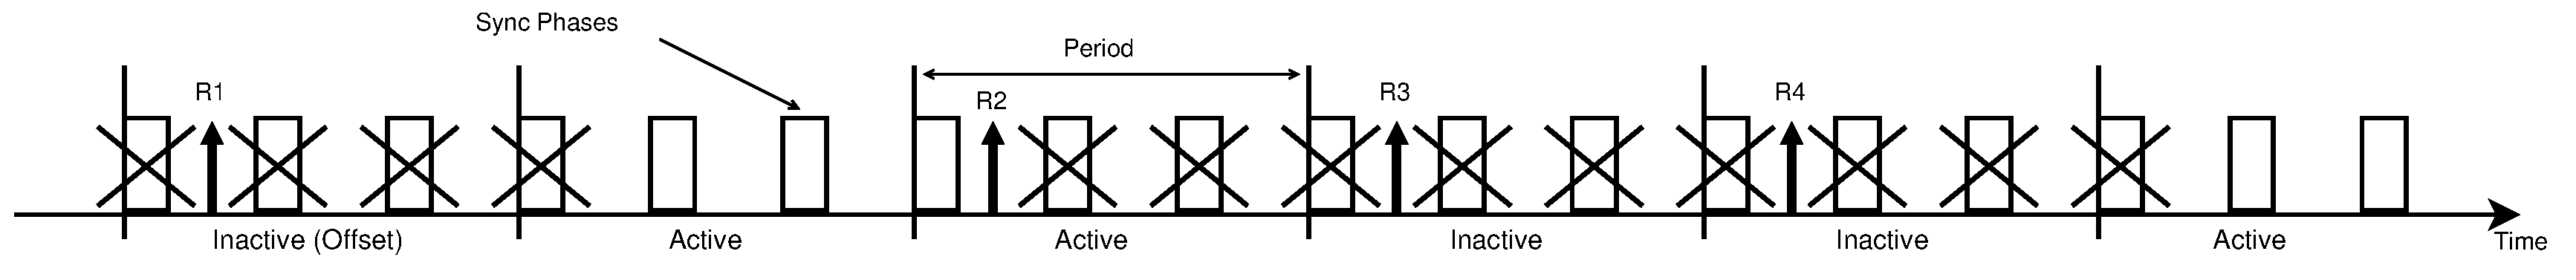
\includegraphics[width=1\textwidth]{parametersphases.eps}
 \end{center}
 \caption{Parameters Example}
 \label{fig:parametersphases}
\end{figure}

In Figure \ref{fig:parametersphases}, it can be seen how the first period is left inactive due to the offsetPhases = 1. Although the period
is inactive, it has an extra report (offsetReportPhases is 0). As reportPhases is 3, the first period of 3 will be an extra report (R1), 
then 2 periods will not have extra report and then another extra report will be scheduled (R3). After the first inactive period, 2 active 
periods come (activePhases = 2). Then 2 inactive periods (inactivePhases = 2) and so on.

In the last active period from an active period group, during the Report Phase the position is calculated (for mode 2) or the \ac{RSSI} 
values are sent (for modes 1 and 4) to the selected \ac{AN} (R2). After this moment, it makes no sense for the \acp{MN} listening to more
Sync Phases, that is why this are crossed out.

It can be also seen that due to offsetSyncPhases = 1, the \ac{MN} is not listening to the first Sync Phase from every active periods 
collection, this is so to make possible, playing with offsetSyncPhases and activePhases, to decide how many Sync Phases will the \ac{MN}
listen to.

Last but not least, as askFrequency = 2, every 2 extra reports, the ASK flag will be activated, in this case in R3. This flag indicates the 
\ac{AN} that the \ac{MN} will ask for some information during the next period, this is made with R4. This request packet does not necessary correspond
to a normal report (modes 1 or 4) or to an extra report but if the period has already one, the same report will be used activating a request
flag.

Make an explanation in detail of the figure, and the protocol with the types of nodes and depending on the parameters before.

Figure \ref{fig:ProtocolPhases} 




Synchronization in the phases.

Centralized vs. Distributed.

Low number of VIP nodes.

Too much time listening to transmit, reduce cases with CSMA when battery is critic using broadcasts from nodes.

As it was seen, \ac{OLP} and \ac{LPL} protocols, are based in \ac{RSSI} values
This work is also based in localization using \ac{RSSI} values, although this work just proposes a framework for the protocol and does not try 
to locate any
node 


\section{Sync Phase detail}

Explain syncPacketsPerSyncPhase parameter.
